% Created by tikzDevice version 0.10.1 on 2017-03-14 14:20:47
% !TEX encoding = UTF-8 Unicode
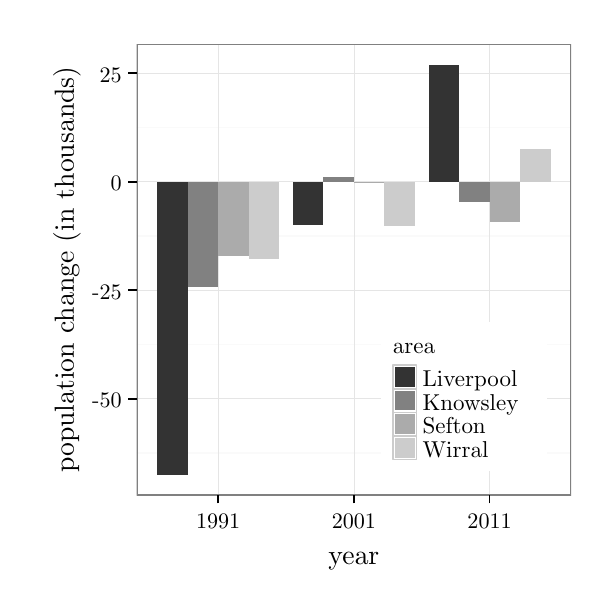
\begin{tikzpicture}[x=1pt,y=1pt]
\definecolor{fillColor}{RGB}{255,255,255}
\path[use as bounding box,fill=fillColor,fill opacity=0.00] (0,0) rectangle (202.36,202.36);
\begin{scope}
\path[clip] (  0.00,  0.00) rectangle (202.36,202.36);
\definecolor{drawColor}{RGB}{255,255,255}
\definecolor{fillColor}{RGB}{255,255,255}

\path[draw=drawColor,line width= 0.6pt,line join=round,line cap=round,fill=fillColor] (  0.00,  0.00) rectangle (202.36,202.36);
\end{scope}
\begin{scope}
\path[clip] ( 39.40, 33.48) rectangle (196.36,196.36);
\definecolor{fillColor}{RGB}{255,255,255}

\path[fill=fillColor] ( 39.40, 33.48) rectangle (196.36,196.36);
\definecolor{drawColor}{gray}{0.98}

\path[draw=drawColor,line width= 0.6pt,line join=round] ( 39.40, 48.66) --
	(196.36, 48.66);

\path[draw=drawColor,line width= 0.6pt,line join=round] ( 39.40, 87.87) --
	(196.36, 87.87);

\path[draw=drawColor,line width= 0.6pt,line join=round] ( 39.40,127.08) --
	(196.36,127.08);

\path[draw=drawColor,line width= 0.6pt,line join=round] ( 39.40,166.29) --
	(196.36,166.29);
\definecolor{drawColor}{gray}{0.90}

\path[draw=drawColor,line width= 0.2pt,line join=round] ( 39.40, 68.27) --
	(196.36, 68.27);

\path[draw=drawColor,line width= 0.2pt,line join=round] ( 39.40,107.48) --
	(196.36,107.48);

\path[draw=drawColor,line width= 0.2pt,line join=round] ( 39.40,146.69) --
	(196.36,146.69);

\path[draw=drawColor,line width= 0.2pt,line join=round] ( 39.40,185.90) --
	(196.36,185.90);

\path[draw=drawColor,line width= 0.2pt,line join=round] ( 68.83, 33.48) --
	( 68.83,196.36);

\path[draw=drawColor,line width= 0.2pt,line join=round] (117.88, 33.48) --
	(117.88,196.36);

\path[draw=drawColor,line width= 0.2pt,line join=round] (166.93, 33.48) --
	(166.93,196.36);
\definecolor{fillColor}{gray}{0.20}

\path[fill=fillColor] ( 46.76, 40.88) rectangle ( 57.79,146.69);
\definecolor{fillColor}{RGB}{129,129,129}

\path[fill=fillColor] ( 57.79,108.83) rectangle ( 68.83,146.69);
\definecolor{fillColor}{gray}{0.67}

\path[fill=fillColor] ( 68.83,119.87) rectangle ( 79.87,146.69);
\definecolor{fillColor}{gray}{0.80}

\path[fill=fillColor] ( 79.87,118.63) rectangle ( 90.90,146.69);
\definecolor{fillColor}{gray}{0.20}

\path[fill=fillColor] ( 95.81,130.96) rectangle (106.84,146.69);
\definecolor{fillColor}{RGB}{129,129,129}

\path[fill=fillColor] (106.84,146.69) rectangle (117.88,148.24);
\definecolor{fillColor}{gray}{0.67}

\path[fill=fillColor] (117.88,146.56) rectangle (128.91,146.69);
\definecolor{fillColor}{gray}{0.80}

\path[fill=fillColor] (128.91,130.53) rectangle (139.95,146.69);
\definecolor{fillColor}{gray}{0.20}

\path[fill=fillColor] (144.85,146.69) rectangle (155.89,188.95);
\definecolor{fillColor}{RGB}{129,129,129}

\path[fill=fillColor] (155.89,139.53) rectangle (166.93,146.69);
\definecolor{fillColor}{gray}{0.67}

\path[fill=fillColor] (166.93,132.29) rectangle (177.96,146.69);
\definecolor{fillColor}{gray}{0.80}

\path[fill=fillColor] (177.96,146.69) rectangle (189.00,158.45);
\definecolor{drawColor}{gray}{0.50}

\path[draw=drawColor,line width= 0.6pt,line join=round,line cap=round] ( 39.40, 33.48) rectangle (196.36,196.36);
\end{scope}
\begin{scope}
\path[clip] (  0.00,  0.00) rectangle (202.36,202.36);
\definecolor{drawColor}{RGB}{0,0,0}

\node[text=drawColor,anchor=base east,inner sep=0pt, outer sep=0pt, scale=  0.80] at ( 34.00, 64.96) {-50};

\node[text=drawColor,anchor=base east,inner sep=0pt, outer sep=0pt, scale=  0.80] at ( 34.00,104.17) {-25};

\node[text=drawColor,anchor=base east,inner sep=0pt, outer sep=0pt, scale=  0.80] at ( 34.00,143.38) {0};

\node[text=drawColor,anchor=base east,inner sep=0pt, outer sep=0pt, scale=  0.80] at ( 34.00,182.59) {25};
\end{scope}
\begin{scope}
\path[clip] (  0.00,  0.00) rectangle (202.36,202.36);
\definecolor{drawColor}{RGB}{0,0,0}

\path[draw=drawColor,line width= 0.6pt,line join=round] ( 36.40, 68.27) --
	( 39.40, 68.27);

\path[draw=drawColor,line width= 0.6pt,line join=round] ( 36.40,107.48) --
	( 39.40,107.48);

\path[draw=drawColor,line width= 0.6pt,line join=round] ( 36.40,146.69) --
	( 39.40,146.69);

\path[draw=drawColor,line width= 0.6pt,line join=round] ( 36.40,185.90) --
	( 39.40,185.90);
\end{scope}
\begin{scope}
\path[clip] (  0.00,  0.00) rectangle (202.36,202.36);
\definecolor{drawColor}{RGB}{0,0,0}

\path[draw=drawColor,line width= 0.6pt,line join=round] ( 68.83, 30.48) --
	( 68.83, 33.48);

\path[draw=drawColor,line width= 0.6pt,line join=round] (117.88, 30.48) --
	(117.88, 33.48);

\path[draw=drawColor,line width= 0.6pt,line join=round] (166.93, 30.48) --
	(166.93, 33.48);
\end{scope}
\begin{scope}
\path[clip] (  0.00,  0.00) rectangle (202.36,202.36);
\definecolor{drawColor}{RGB}{0,0,0}

\node[text=drawColor,anchor=base,inner sep=0pt, outer sep=0pt, scale=  0.80] at ( 68.83, 21.47) {1991};

\node[text=drawColor,anchor=base,inner sep=0pt, outer sep=0pt, scale=  0.80] at (117.88, 21.47) {2001};

\node[text=drawColor,anchor=base,inner sep=0pt, outer sep=0pt, scale=  0.80] at (166.93, 21.47) {2011};
\end{scope}
\begin{scope}
\path[clip] (  0.00,  0.00) rectangle (202.36,202.36);
\definecolor{drawColor}{RGB}{0,0,0}

\node[text=drawColor,anchor=base,inner sep=0pt, outer sep=0pt, scale=  1.00] at (117.88,  8.40) {year};
\end{scope}
\begin{scope}
\path[clip] (  0.00,  0.00) rectangle (202.36,202.36);
\definecolor{drawColor}{RGB}{0,0,0}

\node[text=drawColor,rotate= 90.00,anchor=base,inner sep=0pt, outer sep=0pt, scale=  1.00] at ( 16.67,114.92) {population change (in thousands)};
\end{scope}
\begin{scope}
\path[clip] (  0.00,  0.00) rectangle (202.36,202.36);
\definecolor{fillColor}{RGB}{255,255,255}

\path[fill=fillColor] (127.73, 42.02) rectangle (187.82, 95.92);
\end{scope}
\begin{scope}
\path[clip] (  0.00,  0.00) rectangle (202.36,202.36);
\definecolor{drawColor}{RGB}{0,0,0}

\node[text=drawColor,anchor=base west,inner sep=0pt, outer sep=0pt, scale=  0.83] at (132.00, 84.76) {area};
\end{scope}
\begin{scope}
\path[clip] (  0.00,  0.00) rectangle (202.36,202.36);
\definecolor{drawColor}{gray}{0.80}
\definecolor{fillColor}{RGB}{255,255,255}

\path[draw=drawColor,line width= 0.6pt,line join=round,line cap=round,fill=fillColor] (132.00, 71.89) rectangle (140.54, 80.43);
\end{scope}
\begin{scope}
\path[clip] (  0.00,  0.00) rectangle (202.36,202.36);
\definecolor{fillColor}{gray}{0.20}

\path[fill=fillColor] (132.71, 72.60) rectangle (139.82, 79.72);
\end{scope}
\begin{scope}
\path[clip] (  0.00,  0.00) rectangle (202.36,202.36);
\definecolor{drawColor}{gray}{0.80}
\definecolor{fillColor}{RGB}{255,255,255}

\path[draw=drawColor,line width= 0.6pt,line join=round,line cap=round,fill=fillColor] (132.00, 63.36) rectangle (140.54, 71.89);
\end{scope}
\begin{scope}
\path[clip] (  0.00,  0.00) rectangle (202.36,202.36);
\definecolor{fillColor}{RGB}{129,129,129}

\path[fill=fillColor] (132.71, 64.07) rectangle (139.82, 71.18);
\end{scope}
\begin{scope}
\path[clip] (  0.00,  0.00) rectangle (202.36,202.36);
\definecolor{drawColor}{gray}{0.80}
\definecolor{fillColor}{RGB}{255,255,255}

\path[draw=drawColor,line width= 0.6pt,line join=round,line cap=round,fill=fillColor] (132.00, 54.82) rectangle (140.54, 63.36);
\end{scope}
\begin{scope}
\path[clip] (  0.00,  0.00) rectangle (202.36,202.36);
\definecolor{fillColor}{gray}{0.67}

\path[fill=fillColor] (132.71, 55.53) rectangle (139.82, 62.64);
\end{scope}
\begin{scope}
\path[clip] (  0.00,  0.00) rectangle (202.36,202.36);
\definecolor{drawColor}{gray}{0.80}
\definecolor{fillColor}{RGB}{255,255,255}

\path[draw=drawColor,line width= 0.6pt,line join=round,line cap=round,fill=fillColor] (132.00, 46.28) rectangle (140.54, 54.82);
\end{scope}
\begin{scope}
\path[clip] (  0.00,  0.00) rectangle (202.36,202.36);
\definecolor{fillColor}{gray}{0.80}

\path[fill=fillColor] (132.71, 46.99) rectangle (139.82, 54.11);
\end{scope}
\begin{scope}
\path[clip] (  0.00,  0.00) rectangle (202.36,202.36);
\definecolor{drawColor}{RGB}{0,0,0}

\node[text=drawColor,anchor=base west,inner sep=0pt, outer sep=0pt, scale=  0.83] at (142.70, 72.71) {Liverpool};
\end{scope}
\begin{scope}
\path[clip] (  0.00,  0.00) rectangle (202.36,202.36);
\definecolor{drawColor}{RGB}{0,0,0}

\node[text=drawColor,anchor=base west,inner sep=0pt, outer sep=0pt, scale=  0.83] at (142.70, 64.18) {Knowsley};
\end{scope}
\begin{scope}
\path[clip] (  0.00,  0.00) rectangle (202.36,202.36);
\definecolor{drawColor}{RGB}{0,0,0}

\node[text=drawColor,anchor=base west,inner sep=0pt, outer sep=0pt, scale=  0.83] at (142.70, 55.64) {Sefton};
\end{scope}
\begin{scope}
\path[clip] (  0.00,  0.00) rectangle (202.36,202.36);
\definecolor{drawColor}{RGB}{0,0,0}

\node[text=drawColor,anchor=base west,inner sep=0pt, outer sep=0pt, scale=  0.83] at (142.70, 47.11) {Wirral};
\end{scope}
\end{tikzpicture}
